\documentclass[aspectratio=169, pdf, 8pt, unicode]{beamer}
\usepackage[american,russian]{babel}
\usepackage[default]{sourcesanspro}
\usepackage{tikz}
\usepackage{tikzscale}
\usepackage{float}
\usepackage{graphicx}
\usepackage{pgfplotstable}
\usepackage{caption}
\usepackage{amsmath}
\usepackage{amssymb}
\usepackage{setspace}

\usetikzlibrary{chains,fit,shapes,arrows.meta}

\DeclareCaptionLabelFormat{gostfigure}{Рисунок #2}
\captionsetup[table]{labelsep=endash,justification=justified,singlelinecheck=false,font=normalsize,skip=0pt} 
\captionsetup[figure]{labelformat=gostfigure,labelsep=endash,justification=centering,singlelinecheck=false,font=normalsize} 
\pgfplotsset{compat=1.9}

\mode<presentation> {
\usetheme{Madrid}
}

\setbeamerfont{institute}{size=\normalsize}
\setbeamertemplate{itemize/enumerate body begin}{\large}
\setbeamertemplate{itemize/enumerate subbody begin}{\tiny}

\title[Бакалаврская работа]{Исследование сборки мусора в bitmap-индексах поисковых систем}

\author{Пучков Кирилл}

\institute[МФТИ]{
    Федеральное государственное автономное образовательное учреждение\\ 
    высшего образования\\
    <<Московский физико-технический институт (национальный исследовательский университет)>>\\
    Физтех-школа прикладной математики и информатики\\
    Кафедра теоретической и прикладной информатики\\
\vspace{0.5cm}
Научный руководитель --- А. М. Неганов
}

\date{Москва 2021}

\setbeamertemplate{caption}[numbered]

\begin{document}

\begin{frame}
\titlepage
\end{frame}

\begin{frame}
\frametitle{Содержание}
\tableofcontents
\end{frame}

\section{Постановка задачи}

\begin{frame}[fragile]
\frametitle{Постановка задачи}
\begin{figure}[H]
\centering
\caption{553 тысячи статей \textit{New York Times}}
\begin{table}[H]
\centering
\small
\singlespacing
\begin{tabular}{|c|c|}
    \hline
    Возраст ссылок      & Количество <<повисших>> ссылок, \%    \\ \hline
    Последние 3 года    & 6                                     \\ \hline
    С 1998 года         & $\geq$ 72                             \\ \hline
\end{tabular}
\end{table}
\end{figure}
\end{frame}

\begin{frame}[fragile]
\frametitle{Постановка задачи}
\begin{figure}[H]
\centering
\caption{Логическое представление индекса}
\begin{table}[H]
\centering
\small
\singlespacing
\begin{tabular}{|c|c|c|c|c|c|c|c|c|c|}
    \hline
                &\multicolumn{3}{c|}{block1}&\multicolumn{3}{c|}{block2}& \ldots \\ \hline
                & doc1  & doc2  & doc3      & doc4  & doc5      & doc6  & \ldots \\ \hline
    feature 1   & 0     & 0     & 0         & 1     & 1         & 1     & \ldots \\ \hline
    feature 2   & 1     & 0     & 1         & 0     & 1         & 1     & \ldots \\ \hline
    \vdots      & \vdots& \vdots& \vdots    & \vdots& \vdots    &\vdots & $\ddots$ \\ \hline
\end{tabular}
\label{index}
\end{table}
\end{figure}
\end{frame}

\begin{frame}[fragile]
\frametitle{Постановка задачи}
\begin{figure}[H]
\centering
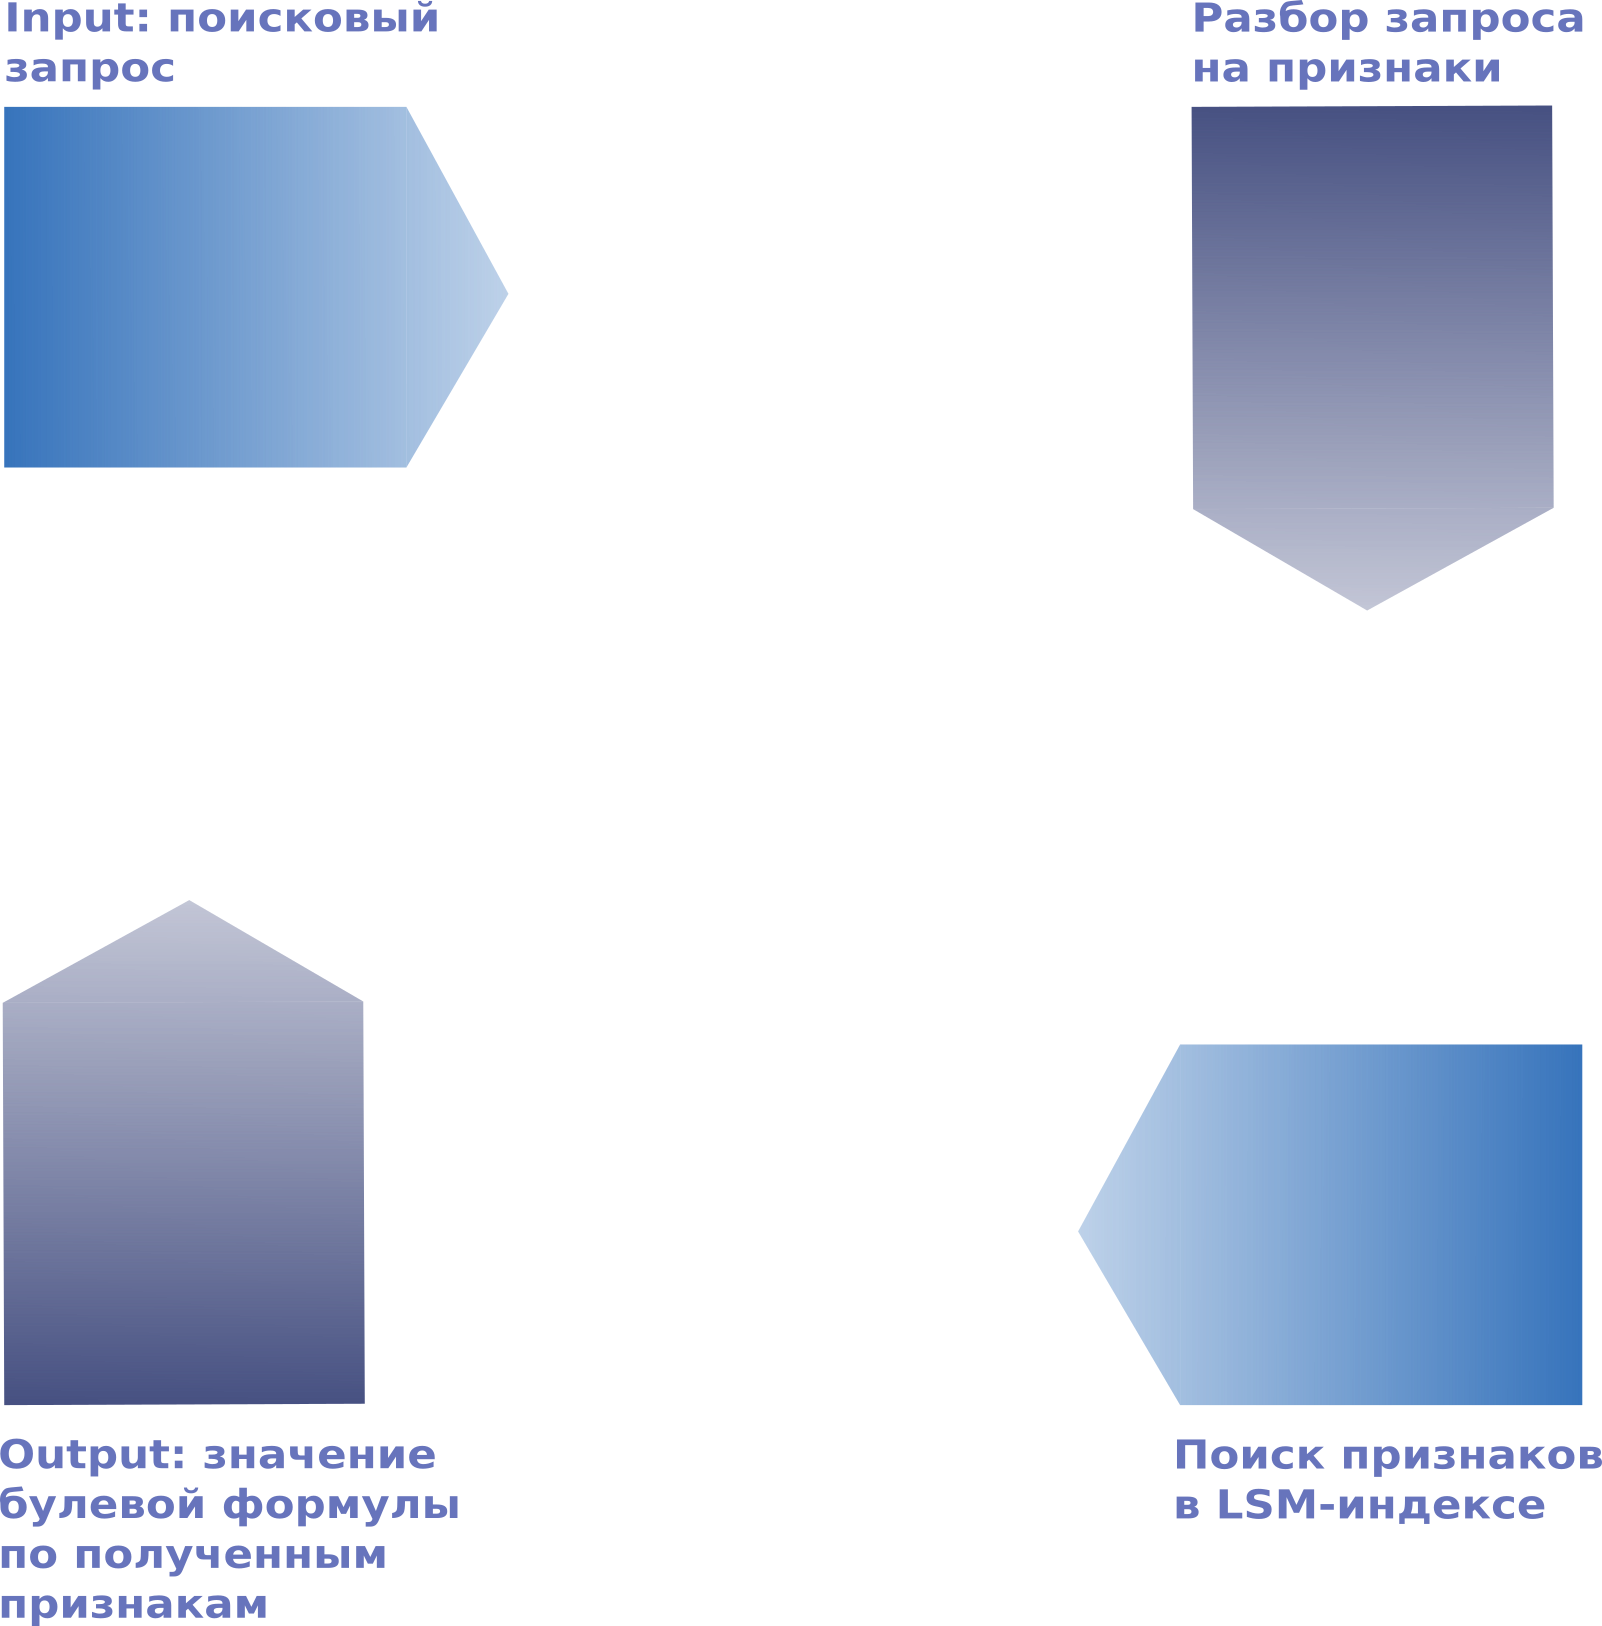
\includegraphics[width=0.4\textwidth]{fig/parser.png}
\caption{Разбор поискового запроса}
\end{figure}
\end{frame}

\begin{frame}[fragile]
    \frametitle{Постановка задачи}
    {\large Задачи:}
    \vspace{5mm}
    \begin{enumerate}
    \item Исследовать существующие методы сбора мусора данных в поисковых системах и структурах данных.
    \vspace{5mm}
    \item Произвести анализ иных свойств метода, его преимуществ и недостатков.
    \vspace{5mm}
    \item Программно реализовать метод.
    \vspace{5mm}
    \item Сравнить скорость работы алгоритма с методом мгновенного удаления.
    \end{enumerate}
    \end{frame}

\section{Сбор мусора}

\begin{frame}[fragile]
\frametitle{Сбор мусора}

Карта \textit{danglingBmap} отображает блоки в индексе в битмапы,
содержащие биты повисших документов в блоке. В случае, если число повисших документов в блоке превышает пороговое — считаем блок <<мусорным>>.

\begin{block}{Алгоритм сбора мусора}
    \begin{enumerate}
        \item Для каждого блока в карте \textit{danglingBmap} проверить, превышает ли мощность битмапы допустимое пороговое значение для индекса.
        \item Для каждого такого блока выполнить операцию НЕ И с битмапой, полученной из первичного индекса. Полученная битмапа не содержит удаленных документов. Оставшиеся документы проверить во вторичном индексе на актуальность.
        \item Присвоить живым документам новый \textit{docId} и обновить на них ссылку во вторичном индексе.
        \item Продублировать значения битов в битмапах для новых \textit{docId} в первичном индексе.
        \item Удалить блок данных для старых \textit{docId}.
        \item В конце сбора мусора обнулить danglingBmap для <<мусорных>> блоков.
    \end{enumerate}
\end{block}
\end{frame}

\begin{frame}[fragile]
\frametitle{Сбор мусора}

Оценим теоретически возможное уменьшение числа блоков и, как следствие, ускорение поиска после сбора мусора.

\begin{block}{Теоретическое ускорение}
    Общий размер индекса
    \begin{equation}
        \left\lceil\frac{N}{\tau}\right\rceil \cdot F = \psi
    \end{equation}
    блоков, где $N$ — число добавленных документов, $\tau$ — размер блока, а
    $F$ — среднее число признаков на 1 документ.

    Таким образом, в случае плотных битмап, последовательного удаления и достаточного количества удаленных элементов $\frac{D}{\tau} > d$ ожидается, что в индексе образуется
    \begin{equation}
        \left\lceil\frac{D}{\tau}\right\rceil \cdot F = \zeta
    \end{equation}
    мусорных блоков, где $D$ — общее число удаленных документов, $d$ — пороговое <<мусорное>> значение для блока.

    Тогда после удаления <<мусорных>> блоков и завершения фоновых операций
    записи и слияния ожидается ускорение операции поиска признаков в 
    \begin{equation}
        \frac{\psi - \zeta}{\psi}
    \end{equation}
    раз.
\end{block}
\end{frame}

\section{<<Мгновенное>> удаление}

\begin{frame}[fragile]
\frametitle{<<Мгновенное>> удаление}

Создадим дополнительную структуру данных, карту \textit{doc2FieldFeature} , для отображения документов в набор их признаков и значений.

\begin{block}{Алгоритм слияния}
    \begin{enumerate}
        \item Результирующая битмапа удаленных документов == побитовое ИЛИ битмап удаленных документов для старого и нового элементов.
        \item Главная битмапа результирующего элемента == побитовое ИЛИ нового и старого элементов индекса. Далее к полученной битмапе
        применяется операция побитового НЕ И с полученной выше битмапой удаленных документов.
    \end{enumerate}
\end{block}
\end{frame}

\section{Экспериментальное исследование}

\begin{frame}[fragile]
\frametitle{Экспериментальное исследование}
\setstretch{1.5}

\begin{enumerate}
    \item Сравнить время поиска первого вхождения ключа до удаления,
    после сбора мусора и после <<мгновенного>> удаления.
    \vspace{4mm}
    \item Сравнить время поиска всех вхождений ключа до удаления,
    после сбора мусора и после <<мгновенного>> удаления.
    \vspace{4mm}
    \item Измерить время работы алгоритма сбора мусора и алгоритма
    «мгновенного» удаления.
    \vspace{4mm}
    \item Исследовать зависимость количества записей и слияний с внешней памятью.
\end{enumerate}
\end{frame}

\begin{frame}[fragile]
    \frametitle{Экспериментальное исследование}
    \setstretch{1.5}
{\large Сценарии поиска:}
    \vspace{4mm}
\begin{enumerate}
    \item Запрос по всем вхождениям заданного ключа для фиксированного числа
    добавленных элементов $N$ и меняющегося размера блока битмапы $2^{x}$.
    \vspace{4mm}
    \item Запрос по первому вхождению заданного ключа для фиксированного числа
    добавленных элементов $N$ и меняющегося размера блока битмапы $2^{x}$.
    \vspace{4mm}
    \item Запрос по всем вхождениям заданного ключа для меняющегося числа добавленных
    элементов $N$.
\end{enumerate}
\end{frame}

\begin{frame}[fragile]
\frametitle{Запрос по всем вхождениям ключа при фиксированном числе добавленных
документов и меняющемся размере блока}
\begin{figure}[H]
\centering
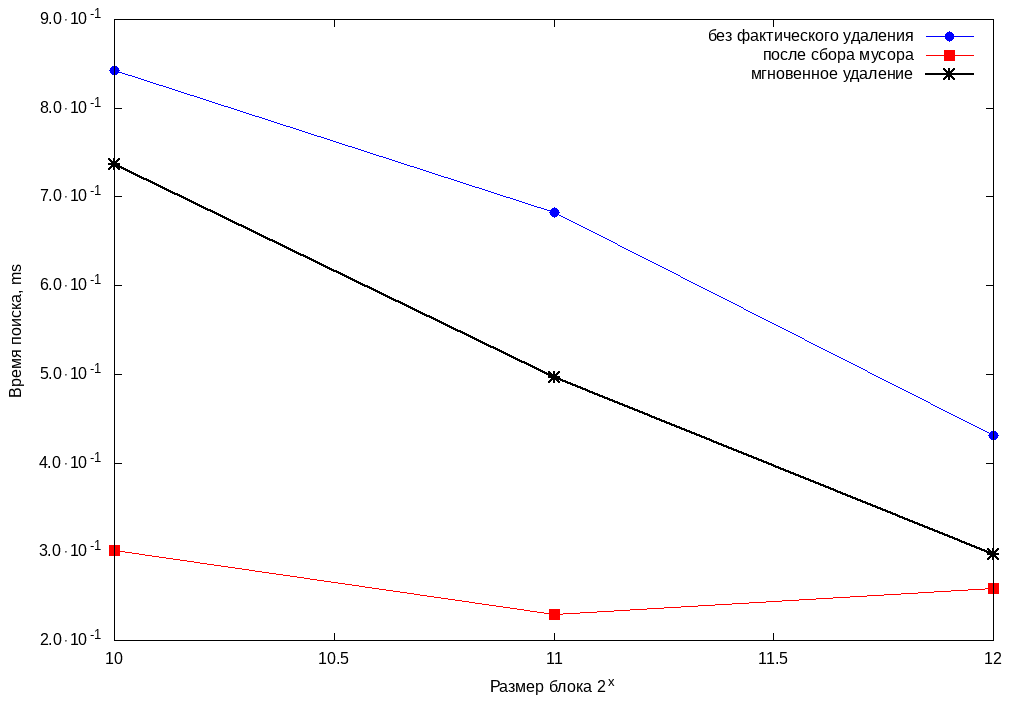
\includegraphics[width=0.5\textwidth]{fig/limit_1e6/1e5/to.png}
\caption{Зависимость времени поиска признака \textit{to} от размера блока для $10^5$ добавленных документов}
\end{figure}
\end{frame}

\begin{frame}[fragile]
\frametitle{Запрос по первому вхождению ключа при фиксированном числе
добавленных документов и меняющемся размере блока}
\begin{figure}[H]
\centering
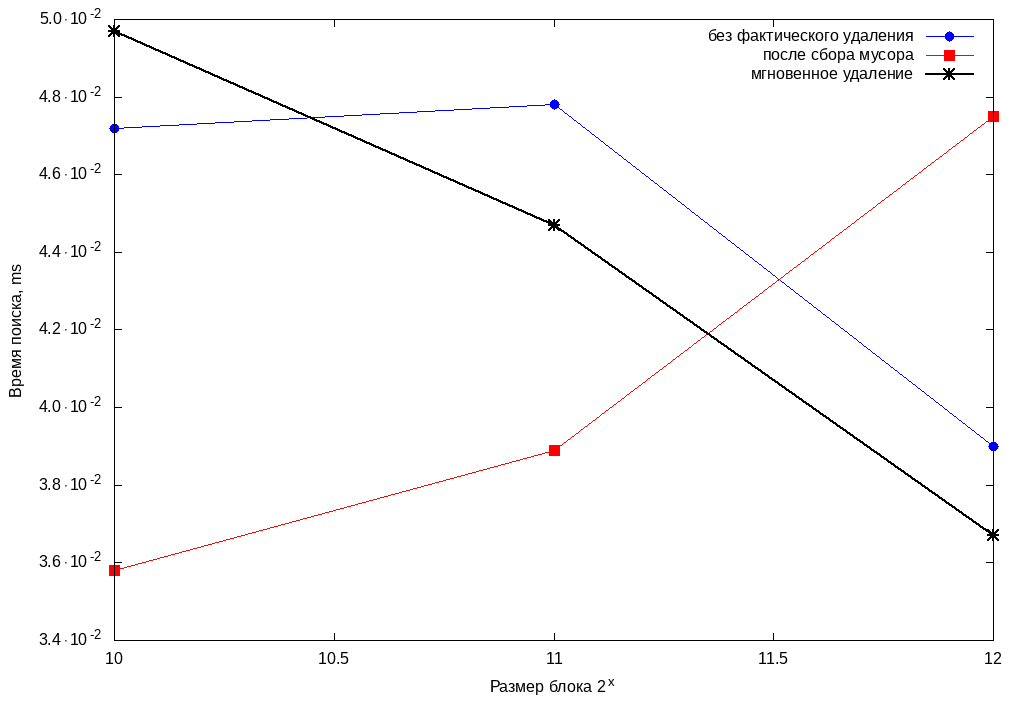
\includegraphics[width=0.5\textwidth]{fig/limit_1/1e5/to.png}
\caption{Зависимость времени поиска признака \textit{to} от размера блока для $10^5$ добавленных документов}
\end{figure}
\end{frame}

\begin{frame}[fragile]
\frametitle{Запрос по всем вхождениям признака для меняющегося числа
добавленных элементов}
\begin{figure}[H]
\centering
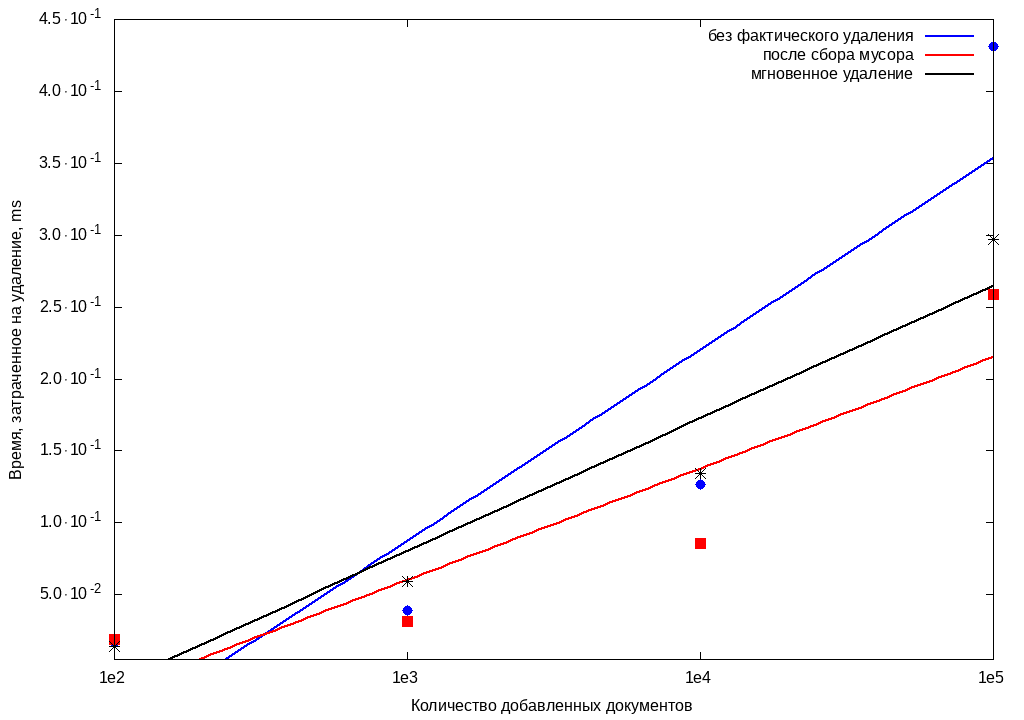
\includegraphics[width=0.5\textwidth]{fig/to.png}
\caption{Зависимость времени поиска \textit{to} от количества добавленных документов}
\end{figure}
\end{frame}

\begin{frame}[fragile]
\frametitle{Запрос по всем вхождениям признака для меняющегося числа
добавленных элементов}
\begin{figure}[H]
\centering
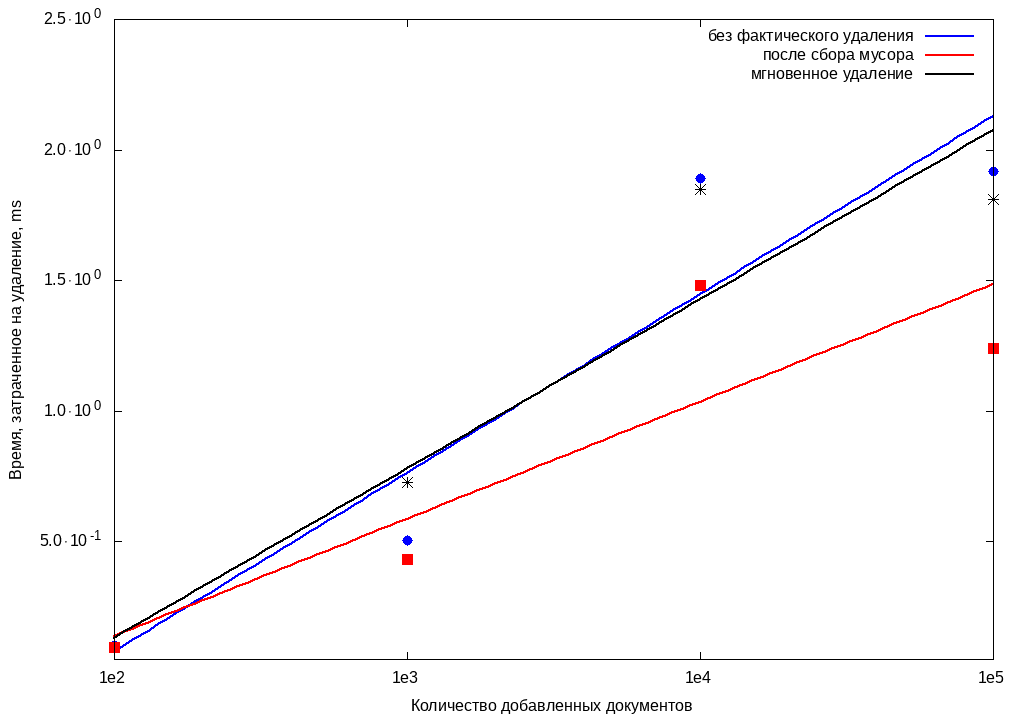
\includegraphics[width=0.5\textwidth]{fig/from.png}
\caption{Зависимость времени поиска \textit{from} от количества добавленных документов}
\end{figure}
\end{frame}

\begin{frame}[fragile]
\frametitle{Сравнение времени работы алгоритма сбора мусора и алгоритма
«мгновенного» удаления}
\begin{figure}[H]
\centering
\begin{minipage}[h]{0.475\linewidth}
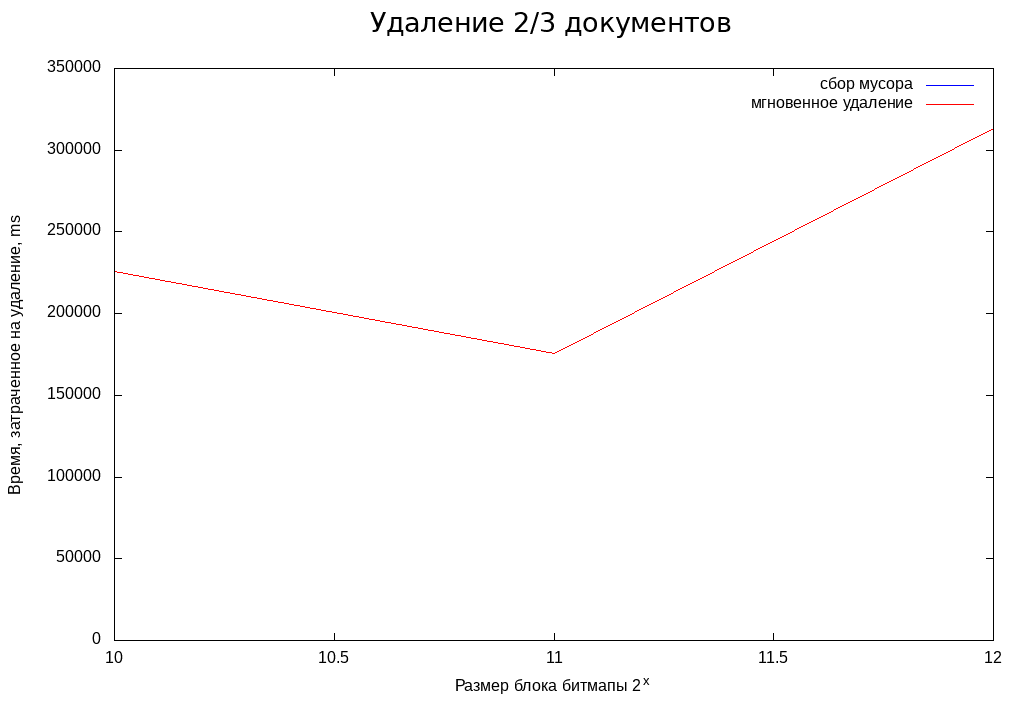
\includegraphics[width=1\textwidth]{fig/time_1e5.png}
\caption{Зависимость времени работы алгоритма от размера блока}
\end{minipage}
\hfil
\begin{minipage}[h]{0.35\linewidth}
\caption{Время работы алгоритмов для
    $10^5$ документов, мс}
\begin{table}[H]
      \centering
      \small
      \singlespacing
      \begin{tabular}{|p{1.5cm}|p{1.5cm}|p{2cm}|}
            \hline
            Размер блока & Сбор мусора                & <<Мгновенное>> удаление \\ \hline \hline
            10           & 2.54e-01                   & 2.26e+05              \\ \hline
            11           & 2.55e-01                   & 1.76e+05              \\ \hline
            12           & 2.54e-01                   & 3.14e+05              \\ \hline
            13           & 2.55e-01                   & 2.36e+05              \\ \hline
            14           & 2.55e-01                   & 2.33e+05              \\ \hline
            15           & 2.54e-01                   & 1.83e+05              \\ \hline
\end{tabular}
\end{table}
\end{minipage}
\end{figure}
\end{frame}

\begin{frame}[fragile]
\frametitle{Сравнение времени работы алгоритма сбора мусора и алгоритма
«мгновенного» удаления}
\begin{figure}[H]
\centering
\begin{minipage}[h]{0.475\linewidth}
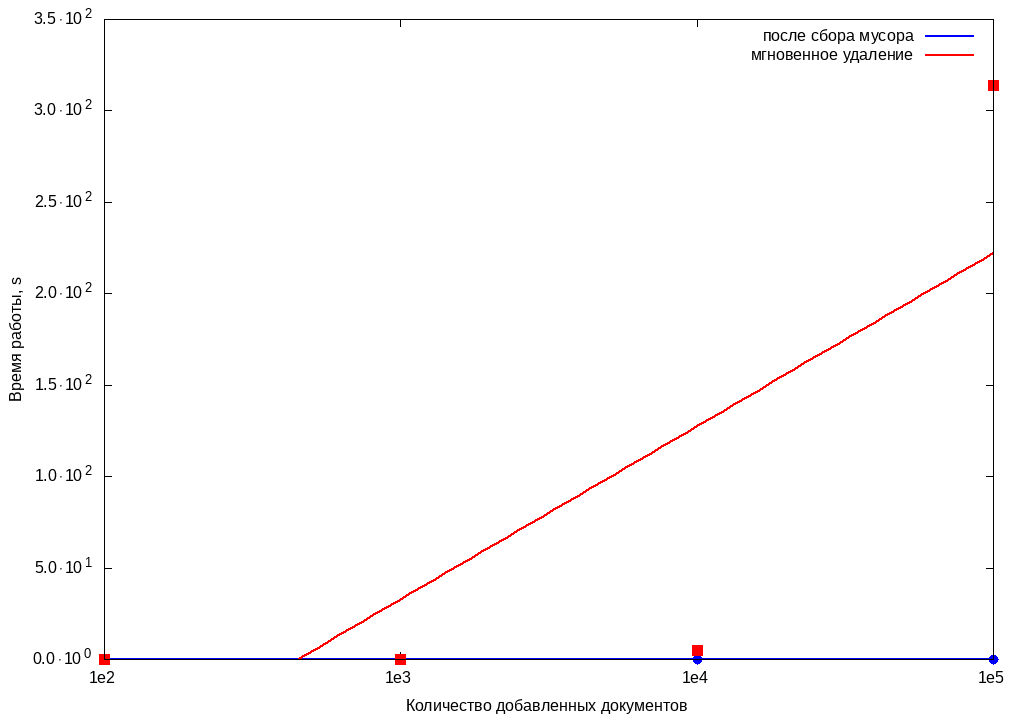
\includegraphics[width=1\textwidth]{fig/time.png}
\caption{Зависимость времени работы алгоритма от количества добавленных документов}
\end{minipage}
\hfil
\begin{minipage}[h]{0.35\linewidth}
\caption{Время работы алгоритмов, с}
\begin{table}[H]
      \centering
      \small
      \singlespacing
      \begin{tabular}{|p{1.5cm}|p{1.5cm}|p{2cm}|}
        \hline
        Число документов & Сбор мусора                & <<Мгновенное>> удаление \\ \hline \hline
        $10^2$           & 3.60e-02                   & 1.71e-02              \\ \hline
        $10^3$           & 1.47e-01                   & 1.79e-01              \\ \hline
        $10^4$           & 2.54e-04                   & 5.11e+00              \\ \hline
        $10^5$           & 2.54e-04                   & 3.14e+02              \\ \hline
\end{tabular}
\end{table}
\end{minipage}
\end{figure}
\end{frame}

\begin{frame}[fragile]
\frametitle{Сравнение количества операций записи и слияния для различного числа
добавленных документов}
\begin{figure}[H]
\centering
\hfil
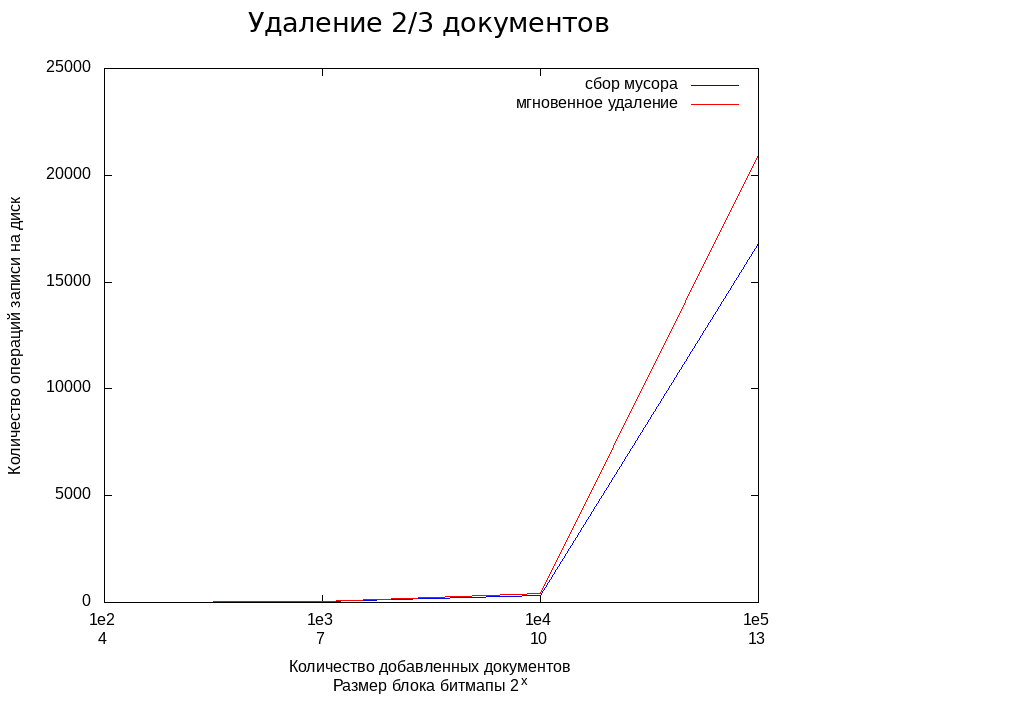
\includegraphics[width=0.6\textwidth]{fig/writecalls.png}
\caption{Зависимость количества операций записи на диск от количества добавленных документов}
\end{figure}
\end{frame}

\begin{frame}[fragile]
\frametitle{Сравнение количества операций записи и слияния для различного числа
добавленных документов}
\begin{figure}[H]
\centering
\hfil
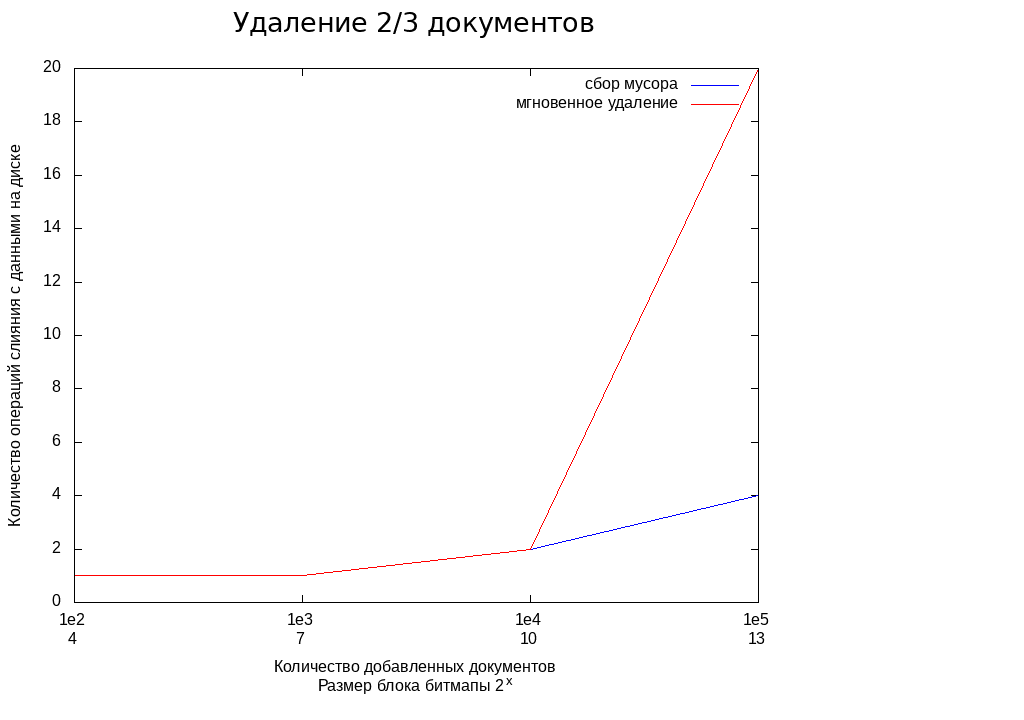
\includegraphics[width=0.6\textwidth]{fig/merges.png}
\caption{Зависимость количества слияний с диском от количества добавленных документов}
\end{figure}
\end{frame}

\section{Выводы}

\begin{frame}[fragile]
\frametitle{Выводы}
\setstretch{2}
\begin{enumerate}
\item Время поиска по первому вхождению ключа уменьшается после сборки мусора.
\item Время поиска по всем вхождениям ключа уменьшается после сборки .
\item Время поиска после сборки мусора меньше по сравнению с <<мгновенным>>
удалением.
\item Длительность сбора мусора в десятки тысяч раз меньше длительности
<<мгновенного>> удаления.
\item Алгоритм сбора мусора не менее эффективен в плане обращений к диску, чем
алгоритм <<мгновенного>> удаления.
\end{enumerate}
\end{frame}

\section{Направления дальнейшего исследования}

\begin{frame}[fragile]
\frametitle{Направления дальнейшего исследования}
\setstretch{2}
\begin{enumerate}
\item Оценка приоритета блоков при очистке.
\item Теоретическая оценка размера метаданных индекса при более общих
исходных предположениях.
\item Детальное построение параллелизуемого алгоритма.
\end{enumerate}
\end{frame}

\end{document}